\subsection{Erweiterung der Generalisierungshierarchie}
\label{sec:Kap-9.2.3}

Sollen Generalisierungshierarchien durch neue Klassen ergänzt werden, wird häufig nur an die Bildung neuer Unterklassen gedacht. Dies ist aber keineswegs immer sinnvoll. Gelegentlich empfiehlt sich die Einführung neuer Oberklassen, wenn Unterklassen einige Eigenschaften der Oberklasse nicht benötigen oder nicht konform verwenden können.

Schauen wir uns noch einmal Abbildung~\ref{fig:angestellter_vorgesetzter.pdf} an: 

Die Klasse \sttpUMLText{Vorgesetzter} sollte keine Unter\-klasse der Klasse \sttpUMLText{Angestellter} sein, da die Operation \sttpUMLText{setzeStellenbezeichnung()} in \sttpUMLText{Vorgesetzter} nicht konform zur entsprechenden Operation in \sttpUMLText{Angestellter} ist. Besser ist die Definition einer neuen Klasse \sttpUMLText{Firmenangehöriger}, von der die Klassen \sttpUMLText{Angestellter} und \sttpUMLText{Vorgesetzter} Unterklassen sind (s.~Abb.~\ref{fig:angestellter_vorgesetzter_firmenangehoeriger.pdf}).

\vspace{\baselineskip} %%% für Druck
\vspace{\baselineskip} %%% für Druck

\begin{figure}[h!]
	\centering
	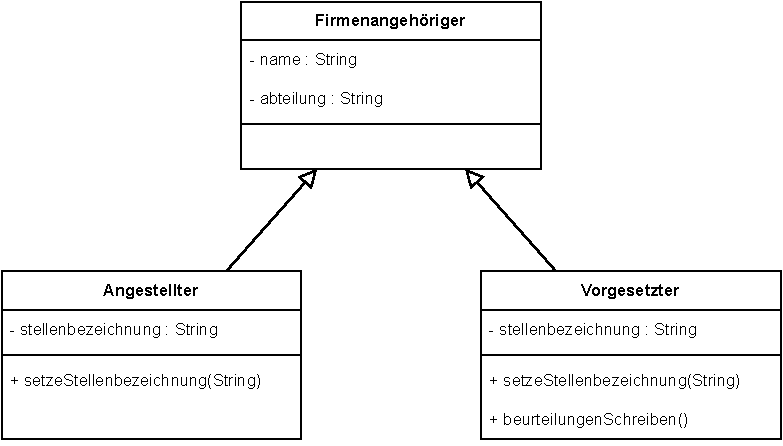
\includegraphics{Bilder/Kapitel-9/angestellter_vorgesetzter_firmenangehoeriger.pdf}
	\vspace{\baselineskip} %%% für Druck
	\caption{Unterklassen derselben Oberklasse}
	\label{fig:angestellter_vorgesetzter_firmenangehoeriger.pdf}
\end{figure}

\vspace{\baselineskip} %%% für Druck
\vspace{\baselineskip} %%% für Druck

Ziel bei der Bildung neuer Unterklassen ist, möglichst wenige Operationen zu überschreiben, damit der Implementations- und Testaufwand schwach ist. Um dieses Ziel zu erreichen, sollte schon bei der Definition der Oberklasse an später zu definierende Unterklassen gedacht werden.

Betrachten wir ein weiteres Beispiel. Gegeben sei die Klasse \sttpUMLText{LinkedList} mit Operationen zum Einfügen und Löschen von Elementen und zum Durchsuchen der Liste (s.~Abb.~\ref{fig:linked_list}):

\pagebreak %%% für Druck

\vspace*{\baselineskip} %%% für Druck

\begin{figure}[h!]
	\centering
	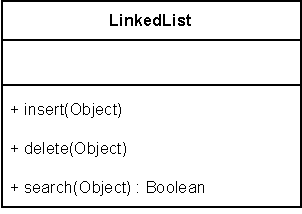
\includegraphics{Bilder/Kapitel-9/linked_list.pdf}
	\vspace{\baselineskip} %%% für Druck
	\caption{Die Klasse \sttpUMLText{LinkedList}}
	\label{fig:linked_list}
\end{figure}

\vspace{\baselineskip} %%% für Druck

Ein verketteter Ring unterscheidet sich von einer verketteten Liste nur dadurch, dass das letzte Element wieder einen Verweis auf das erste Element enthält. Definiert man eine Klasse \sttpUMLText{LinkedRing} als Unterklasse von \sttpUMLText{LinkedList}, so muss man alle drei Operationen vollständig neu implementieren, da Listendurchläufe in den geerbten Operationen nicht mehr terminieren. Hätte \sttpUMLText{LinkedList} dagegen eine \sttpUMLText{protected}-Operation \sttpUMLText{atEnd(Object):boolean}, welche die Abfrage auf das Listenende realisiert und von allen anderen Operationen verwendet wird, so muss nur die Operation \sttpUMLText{atEnd()} in der Klasse \sttpUMLText{LinkedRing} reimplementiert werden.

Klassen sollten also so definiert werden, dass sie für Unterklassenbildung offen, aber für unkontrollierte Zugriffe geschlossen sind (\textit{Open-Closed-Principle}).